The CORDET Framework defines the Application State Machine of figure \ref{fig:ApplicationSM} to model the start-up and shutdown logic of an application. 

When the application is created, the Application State Machine is in state START\_UP. 
In this state, the \textit{Application Start-Up Procedure} is executed. 
This procedure is entirely defined at application level but is subject to two constraints: (a) the procedure must include the instantiation, initialization and configuration of all components subject to early instantiation, and (b) the procedure may only terminate if successful configuration of all components subject to early instantiation is confirmed (i.e. if all these components are in state CONFIGURED). 

Normal operation takes place in state NORMAL. 
In particular, the services provided by an application to its users are only guaranteed to be available when the application is in state NORMAL and it is only from this state that the application makes use of the services provided by other applications. 
Thus, in state NORMAL, an application may assume that its service interfaces are all operational.

An application can be reset by sending command \texttt{Reset} to its \textit{Application State Machine}. This causes a transition to state RESET where the \textit{Application Reset Procedure} is executed. This procedure is entirely defined at application level but is subject to two constraints: (a) the procedure must include the sending of the \texttt{Reset} command to all currently instatiated components, and (b) the procedure may only terminate if all currently instantiated components are in state CONFIGURED.

It follows from the logic outlined above that, when the application is in state NORMAL, all its statically instantiated components are guaranteed to be correctly configured (i.e. they are guaranteed to be in state CONFIGURED).

The \textit{Application Start-Up Procedure} and the \textit{Application Reset Procedure} will normally share much behaviour but they may not coincide because there may be some actions which are only executed once when an application is started up (such as, for instance, the initialization of all application components).

Finally, the orderly shutdown of an application is performed by sending command \texttt{Shutdown} to the \textit{Application State Machine}. This triggers a transition to state SHUTDOWN where the \textit{Application Shutdown Procedure} is executed. This procedure is entirely defined at application level but is subject to one constraint: the procedure must include the sending of the \texttt{Shutdown} command to all currently instantiated components. 

\begin{figure}[ht]
 \centering
 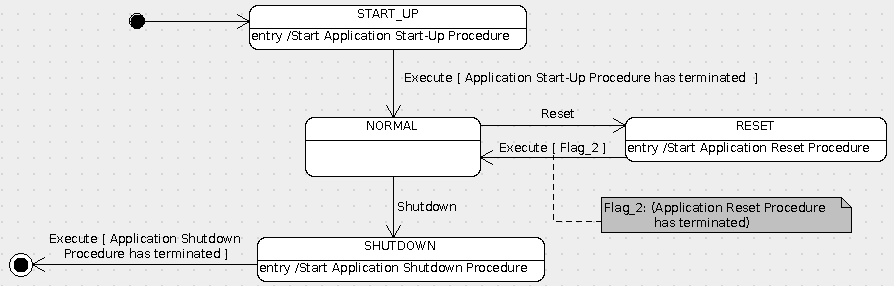
\includegraphics[scale=0.4,keepaspectratio=true]{ApplicationSM.png}
 \caption{Application State Machine}
 \label{fig:ApplicationSM}
\end{figure}

Applications may (and normally will) define embedded state machines in the states shown in figure \ref{fig:ApplicationSM}. In particular, applications normally have several operational states which would appear as sub-states of NORMAL.
